\begin{frame}{Introduction}
  \begin{itemize}
    \item Consider a statistical model 
    parameterised by $\btheta = (\theta_1,\dots,\theta_p)^\top$ 
    for which we have observations $\by = \{y_1, \dots, y_n\}$ and also some latent variables $\bz = \{z_1, \dots, z_m\}$.
    \pause  
    \item Want to evaluate the intractable integral
    \[
      I := \int p(\by|\bz)p(\bz) \d\bz \ \rlap{\color{gray!60} $= p(\by)$}
    \]
    \vspace{-0.8em}
    \begin{itemize}
      \item Frequentist likelihood maximisation {\color{gray!60} $\argmax_\theta \log p(\by|\theta)$} \vspace{0.2em}
      \item Bayesian posterior analysis {\color{gray!60} $p(\bz|\by)=p(\by,\bz)/p(\by)$}
%      \item etc.
    \end{itemize}
%    \pause
%    \item Possible ways: quadrature methods, Laplace approximation, MCMC
    \pause
    \item Variational inference approximates the ``posterior'' $p(\bz|\by)$ by a tractably close distribution in the Kullback-Leibler sense.
    \item<4-> Advantages:
    \begin{itemize}
      \item Computationally fast
      \item Convergence easily assessed
      \item Works well in practice
    \end{itemize}
  \end{itemize}
\end{frame}

\begin{frame}{In the literature}
  \vspace{-12pt}
  \begin{figure}[h]
    \hspace{-15pt}{\color{white} a}
    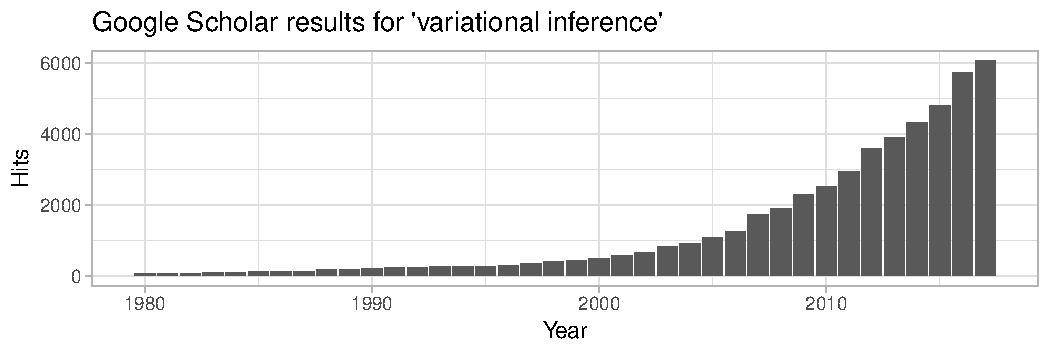
\includegraphics[scale=0.65]{google_scholar}
  \end{figure}
  \vspace{-15pt}
  \begin{itemize}
    \item Well known in machine learning, slowly encroaching other fields.
    \pause
    \item Applications \citep{blei2017variational}:
    \begin{itemize}\footnotesize
      \item Computer vision and robotics {\color{gray!65}(image denoising, tracking, recognition)}   
      \item Natural language processing and speech recognition {\color{gray!65}(topic modelling)}
      \item Social statistics {\color{gray!65}(probit models, latent class models, variable selection)}   
      \item Computational biology {\color{gray!65}(phylogenetic hidden Markov models, population genetics, gene expression analysis)}
      \item Computational neuroscience {\color{gray!65}(autoregressive processes, hierarchical models, spatial models, artificial neural networks)}
    \end{itemize}
  \end{itemize}
\end{frame}

\begin{frame}{Introductory texts}
  \begin{itemize}
    \item \fullcite{blei2017variational}
    \item \fullcite{Bishop2006}
    \item \fullcite{Murphy1991}
    \item \fullcite{beal2003variational}
    \item \fullcite{jamil2018phdthesis}
  \end{itemize}
\end{frame}

\subsection{Idea}

\begin{frame}[label=idea]{Idea}
  \blfootnote{\fullcite{bleiyoutube}}
  \vspace*{-35pt}
  \begin{center}\begin{tikzpicture}
    \draw[draw=none] (0,0) ellipse (4cm and 2.2cm);
    \draw[draw=none] (-0.8,-0.5) to [curve through={(-2,0) .. (-2,-0.8) .. (1,-0.8) .. (-1,1.5) .. (0,1.5) ..(0.3,0.1) .. (0.5,1.5) .. (2,0) .. (2.1,-0.1) .. (2.2,1.1) .. (3,0.9)}] (3.317,1.225);  % required to keep everything in place
    \only<1|handout:0>{\node at (-2.8,0.7) {$q(\bz)$};}
  
    \only<1-2>{\fill (4.05,2.1) circle (0pt) node[right,yshift=1] {$p(\bz|\by)$};}
    \only<2->{
      \draw[ultra thick] (0,0) ellipse (4cm and 2.2cm);
      \node at (-2.8,0.7) {$q(\bz;\nu)$};
    }   
     
    \only<4->{\draw[thick,colred] (-0.8,-0.5) to [curve through={(-2,0) .. (-2,-0.8) .. (1,-0.8) .. (-1,1.5) .. (0,1.5) ..(0.3,0.1) .. (0.5,1.5) .. (2,0) .. (2.1,-0.1) .. (2.2,1.1) .. (3,0.9)}] (3.317,1.225);}  % curve using hobby tikz
    \only<3->{\draw[dashed, very thick,black!50] (3.317,1.225) -- (4.05,2.1);}
    \only<4->{\fill (-0.8,-0.5) circle (2.2pt) node[below] {$\nu^{\text{init}}$};}
    \only<3->{\fill (3.317,1.225) circle (2.2pt) node[left,yshift=-1] {$\nu^*$};}
    \only<3->{\fill (4.05,2.1) circle (2.2pt) node[right,yshift=1] {$p(\bz|\by)$};}
    \only<3->{\node[gray] at (4.5,1.4) {$\KL(q\Vert p)$};}
  \end{tikzpicture}\end{center}
  \vspace{-20pt}
  \begin{itemize}
    \item Minimise Kullback-Leibler divergence (\hyperlink{variationalprinc}{using calculus of variations})
    \[
      \KL(q \Vert p) = -\int \log \frac{p(\bz|\by)}{q(\bz)} q(\bz) \d\bz.
    \]
    \item Use $\tilde q(\bz;\nu^*) := \argmin_q \KL(q \Vert p)$ as an approximation to $p(\bz|\by)$.\vspace{0.2em}
%    \item<5-> \textbf{ISSUE}: $\KL(q\Vert p)$ is intractable.
  \end{itemize}
  
%  \begin{textblock*}{3cm}(.982\textwidth,0.718\textheight)%
%    \hyperlink{variationalprinc}{\beamerbutton{aside}}      
%  \end{textblock*}
\end{frame}

\begin{frame}[label=compareemalg]{The Evidence Lower Bound (ELBO)}  
%  \vspace{-3pt}
  \begin{itemize}\setlength\itemsep{0.45em}
    \item Let $q(\bz)$ be some density function to approximate $p(\bz|\by)$. \pause Then the log-marginal density can be decomposed as follows:
    \begin{align*}
      \log p(\by) &= \log p(\by,\bz) - \log p(\bz|\by) \\
      \onslide<3->{
      &= \int \left\{ \log \frac{p(\by,\bz)}{q(\bz)} - \log \frac{p(\bz|\by)}{q(\bz)} \right\} q(\bz) \d \bz  \\    
      }
      \onslide<4->{
      &=  \cL(q) +  \KL(q \Vert p)  \\
      &\geq \cL(q) 
      }   
    \end{align*}
    \item<5-> $\cL$ is referred to as the ``lower-bound'', and it serves as a surrogate function to the marginal.
    \item<5-> Maximising $\cL(q)$ is equivalent to minimising $\KL(q \Vert p)$.
    \item<6-> N.b. Equality in the bound when $q(\bz) \equiv p(\bz|\by)$, and $\KL(q \Vert p)$ vanishes (c.f. EM algorithm).
%    \begin{itemize}\setlength\itemsep{0.4em}
%      \item $\cL(q) = \E_{\bz\sim q}[\log p(\by,\bz)] + H[q(\bz)]$; and
%      \item<7-> Equality in the bound when $q(\bz) \equiv p(\bz|\by)$, and $\KL(q \Vert p)$ vanishes
%    \end{itemize}
  \end{itemize}
\end{frame}

\subsection{Mean-field distributions}

\begin{frame}{Factorised distributions (Mean-field theory)}
  \begin{itemize}
    \item<1-> Maximising $\cL$ over all possible $q$ not feasible. Need some restrictions, but only to achieve tractability.
    \item<1-> Suppose we partition elements of $\bz$ into $M$ disjoint groups $\bz = (\bz_{[1]}, \dots, \bz_{[M]})$, and assume
    \[
      q(\bz) = \prod_{j=1}^M q_j(\bz_{[j]}).
    \]
    \item<2-> Under this restriction, the solution to $\argmax_q \cL(q)$ is
    \begin{align}\label{eq:meanfieldsoln}
      \tilde q_j(\bz_{[j]}) \propto \exp\big(\E_{-j}[\log p(\by,\bz)]\big)
    \end{align}
    for $j \in \{1,\dots,m\}$.
    \item<3-> In practice, these unnormalised densities are of recognisable form (especially if conjugacy is considered).
    \vspace{4pt}
  \end{itemize}
\end{frame}

\subsection{Coordinate ascent algorithm}

\algrenewcommand{\algorithmiccomment}[1]{{\color{gray}\hfill$\triangleright$ #1}}
\begin{frame}[label=cavi]{Coordinate ascent mean-field variational inference (CAVI)}
  \vspace{-3pt}
  \begin{itemize}[<+->]\setlength\itemsep{0.3em}
    \item The optimal distributions are coupled with another, i.e. each $\tilde q_j(\bz_{[j]})$ depends on the optimal moments of $\bz_{[k]}$, $k \in \{1,\dots,M|k \neq j\}$.
    \item One way around this to employ an iterative procedure.
    \item Assess convergence by monitoring the lower bound
    \[
      \cL(q) = \E_{ q}[\log p(\by, \bz)] - \E_{ q}[\log q(\bz)].
    \]
  \end{itemize}
  \vspace{-24pt}
  \onslide<4->{\begin{center}\scalebox{0.9}{\begin{minipage}{\linewidth}
    \begin{algorithm}[H]
    \caption{CAVI}\label{alg:cavi}
    \begin{algorithmic}[1]
      \State \textbf{initialise} Variational factors $q_j(\bz_{[j]})$
      \While{$\cL(q)$ not converged}
      \For{$j = 1,\dots,M$}
      \State $\log q_j(\bz_{[j]}) \gets \E_{-j}[\log p(\by,\bz)] + \const$
      \Comment{from \eqref{eq:meanfieldsoln}}
      \EndFor
      \State $\cL(q) \gets \E_{ q}[\log p(\by, \bz)] - \E_{ q}[\log q(\bz)]$
      \EndWhile
      \State \textbf{return} $\tilde q(\bz) = \prod_{j=1}^M \tilde q_j(\bz_{[j]})$ 
    \end{algorithmic}
    \end{algorithm}
  \end{minipage}}\end{center}}

%  \begin{textblock*}{3cm}(.89\textwidth,1\textheight)%
%    \hyperlink{varex}{\beamerbutton{example}}      
%  \end{textblock*}
\end{frame}
